
%
% CUSTOM THEOREMS (MI)
%
\newtheorem{theorem}{\textbf{Theorem}}
%\newtheorem{observation}[theorem]{\textbf{Observation}}
%\newtheorem{definition}{\textbf{Definition}}
%\newtheorem{proposition}[theorem]{\textbf{Proposition}}
\newtheorem{remark}[theorem]{\textbf{Remark}}
%\newtheorem{lemma}[theorem]{\textbf{Lemma}}

\chapter{Introduction}
%
This dissertation focuses three optimization problems of which common denominator is communication among multiple devices.

The first two topics concern NP-hard combinatorial network optimization problems, and can naturally be formulated as integer linear programs (ILP).
Instances of limited sizes can be solved to optimality using traditional methdos for solving ILP such as Branch and Bound (B\&B).
In case of larger instances, where finding optimal solution is prohibitively time consuming, methods without guarantee of optimality such as heuristic algorithms are employed.
ILP models are also useful whenever the optimality has to be given up due to the excessive instance size.
Continuous relaxations of ILP models help to evaluate quality of a studied inexact method.
The stronger model, the better assessment it provides.
Devising strong ILP models is therefore of our great interest.
%A common optimization criterium in is energy consumption, as the devices are typically heavily energy constrained due to the use batteries as energy sources.
%Another criterium is time during which a communication session takes place.
The cornerstone of the first two problems is a set of devices of fixed locations with the ability of communicating with each other.
The task is always to disseminate a message initiated at certain source devices to the remaining ones while abiding by certain communication rules and restrictions.
In practical applications, there are various optimization criteria in network communication problems.
The first two problems studied herein require minimizing the power consumption and time during which a communication session takes place.

The last problem belongs to the artificial intelligence (AI) world, particularly to the family of multi-robot path planning problems.
The most general variant, cooperative path-finding \cite{silver05} is NP-hard, and assumse a set of agents deployed in an environment.
Each agent is assigned a target location in the environment, and their task is to reach these locations by a simultaneous movement while obeying several rules.
There are three most common optimization criteria \cite{yu13} to be pursued:
\begin{itemize}
	\item Minimum total arrival time - total number of time steps that the agents need before arrivin in their targets.
	\item Minimum makespan - the number of time steps needed by the latest arriving agent
	\item Minimum total distance - total number of moves performed by the agents
\end{itemize}
Various modifications have been proposed in the literature, and they will be discussed in detail in Section \ref{sec:app}.
An extension of the problem considers agents divided into two adversarial teams, where the teams can have either symmetric or asymmetric objectives.
After introducing the adversarial element, the problem becomes PSPACE-hard, like many two player games with alternating turns.
Additional requirement of preserving a communication possibility during the agets' movement has also been studied.

The remainder of this chapter is structured as follows: 
Section~\ref{sec:back} contains an overview of general underlying mathematical and algorithmical tools and methods employed in the attached papers.
In Section~\ref{sec:smt}, we discuss ad-hoc wireless networks and describe several optimization problems in this area.
In particular, we focus on the shared multicast tree problem and provide an insigt into its relation to other similar problems.
Section~\ref{sec:mbt} introduces the minimum broadcast tree problem and discusses other relevant problems.
In Section~\ref{sec:app}, we describe the problems in multi-robot path planning, and summarize their properties.
An emphasis is given to the area protection problem.

%This is the introduction~\cite{deb01, pyprop}\ldots

\section{Background}\label{sec:back}

%\subsection{Notation and Terminology}

\subsection{Graph Terminology}\label{sec:back:graph}

A \emph{graph} $G$ is a pair $(V,E)$ of \emph{vertices} and \emph{edges}, where $E\subseteq {{V}\choose{2}}$.
If this inclusion is an equality, $G$ is said to be \emph{complete}.
A \emph{path} in graph is a sequence of edges connecting a sequence of distinct vertices.
A graph is said to be \emph{connected} if there exists a path between every two vertices, otherwise it is \emph{disconnected}.
A \emph{cycle} of a graph $G$ is a subset of $E$ that form a path such that the first node of the path corresponds to the last. 
If $G$ contains a cycle, $G$ is called, \emph{cyclic}, otherwise it is called \emph{acyclic}.
\begin{definition}
A tree is a graph that is connected and acyclic.
\end{definition}
For a vertex $v\in V$, a \emph{neighbourhood} of $v$ (open neighbourhood), denoted as $N(v)$, is the set of vertices adjacent to $v$.
The size of neighbourhood of $v$ is called a \emph{degree} of $v$.
A \emph{subgraph} of $G=(V,E)$ is a graph $G'=(V',E')$ such that $V'\subseteq V$ and $E'\subseteq E$.
This relation is often written as $G\subseteq G'$.
\begin{definition}
A spanning tree of graph $G=(V,E)$ is a tree $T=(V_T,E_T)$ such that $T\subseteq G$ and $V_T=V$.
\end{definition}

In a \emph{weighted graph} $G=(V,E,w)$, a \emph{weight} or \emph{cost} $w_e$ is associated witch each edge $e\in E$.
A weight of $G$ is $\sum_{e\in E}w(e)$.
A spanning tree of $G$ with minimum weight is called a \emph{minimum spanning tree} of $G$.
Similar concept is used in paths in graphs.
A \emph{shoretst path} from $u$ to $v$ in a weighted graph is a path consisting of edges of minimum sum of weights connecting $u$ and $v$.
\begin{definition}
	For a graph $G=(V,E)$ and a subset of vertices $D\subseteq V$, a Steiner tree of $G$ and $D$ is a tree $T=(V',E')$ such that $T\subseteq G$ and $D\subseteq V'$.
\end{definition}
Analogously in weighted graphs, a \emph{minimum Steiner tree} is a Steiner tree of minimum weight.

If edges have a direction associated with them, we call such a graph a \emph{directed graph}, and its edges are referred to as \emph{arcs}
Let $G=(V,A)$ be a directed graph. 
By \emph{in-degree} and \emph{out-degree} of a vertex $v\in V$ we mean the sizes of sets $|\{(u,v): u\in V, (u,v) \in A\}|$ and $|\{(v,u): u\in V, (v,u) \in A\}|$ , respectively.
An \emph{arborescence} rooted at vertex $r$ is a directed tree with arcs directed from $r$.
A directed graph is \emph{strongly connected}, if for all pair of vertices $u,v\in V$, there is a path from $u$ to $v$ and from $v$ to $u$.

A graph is \emph{planar}, if it can be drawn in a plane without crossing edges.
According to this definition, every tree is planar. 
A graphical representation of a graph $G$ is determined by function $\Phi(G):V\to\mathbb{R}\times\mathbb{R}$ that assigns a coordinate to each node in $V$. 
We say that $\Phi(G)$ is is an \emph{embedding of $G$ in a plane}.
\begin{definition}\label{def:planemb}
The embedding $\Phi(G)$ is planar if it is drawn in such a way that its straight line segments intersect only at their endpoints.
\end{definition}
Clearly, whenever $\phi(G)$ is planar, then also $G$ is planar. 
The opposite implication does not hold in general. 
If $\Phi(G)$ is not planar, any two edges that intersect each other are referred to as \emph{crossing}.

\subsection{Combinatorial Optimization}

Combinatorial optimization (CO) is a part of applied mathematics that taclkes optimization problems over discrete structures.
It combines methods from graph theory, linear programming, combinatorics and the theory of algorithms.
In this section, we briefly introduce main concepts in CO used later in the text.
For a comprehensive rendition of this topic, an interested reader is referred to \cite{wolsey98} and \cite{nemhauser88}.

Combinatorial problems arise in many areas of computer science with a wide range of applications in various industrial disciplines 
such as production scheduling, logistics, communication network design and many more.
The core solving a problem by methods of CO is the identification of a discrete mathematical structure hidden in the problem,
and finding a sufficient abstraction.

CO concerns problems of minimization or maximization of an \emph{objective function} of several variables 
subject to inequality and equality \emph{constraints} and integrality restriction on at least some of the variables.
In this work, both the objective function and constraints are assumed to be linear.
Combinatorial problems are often formulated as \emph{mixed integer linear programs} (MILP) of the standard form
\begin{equation}
\begin{array}{r@{}l}
	\max\limits_{x,y}c^\top x + h^\top y & \\
	\text{subject to}& \\
	  Ax + Gy &\leq b, \\
	  x \in \mathbb{Z}^{n}_+, y & \in\mathbb{R}^{p}_+. 
\end{array}
\end{equation}

The problem instance is specified by the input data $c\in \mathbb{R}^n$, $h \in \mathbb{R}^n$, $A \in \mathbb{R}^{m\times n}$  $G \in\mathbb{R}^{m\times p}$ and $b \in \mathbb{R}^m$.
A MILP that is not in the standard form, for example if the objective is to minimize or if the constraints contain equalities, can be straightforwardly converted into the standard form.
If the integrality constraints are not present, we talk about a \emph{linear program} (LP)


The set of points $S=\{(x_0,y_0):  x_0 \in \mathbb{Z}^{n}_+, y_0  \in\mathbb{R}^{p}_+, Ax_0 + Gy_0 \leq b\}$ is called the \emph{feasible region},  
and a point $(x_0,y_0)\in S$ is referred to as a \emph{feasible point} (feasible solution) with \emph{objective function value} $c^\top x_0 + h^\top y_0$. 
A feasible point $(x^*,y^*)$ is called an \emph{optimal solution} if for every feasible points $(x_0,y_0)$ we have that $c^\top x_0 + h^\top y_0 \leq c^\top x^* + h^\top y^*$. 
Expression $c^\top x^* + h^\top y^*$ is then called the \emph{optimal value}. 

\subsubsection{Relaxation and Bounds}

\begin{definition}
	Let $S\subseteq \mathbb{R}^n$ and $\mathcal{F}$ be a MILP $\max\{f(x):x\in S\}$.
	The problem $\mathcal{R}: \max\{g(x):x\in T\}$ is a relaxation of $\mathcal{F}$ if and only if
	\begin{enumerate}
		\item $T\supseteq S$, and
		\item $g(x)\geq f(x) \forall x\in S$.
	\end{enumerate}
\end{definition}


Let $z^*$ and $\underline{z}$ be the optimal value of a MILP and its relaxation, respectively. 
Further, let $\bar{z}$ be the objective function value of some feasible point.
Then, $\underline{z}\leq z^* \leq \bar{z}$.
Values $\underline{z}$ and $\bar{z}$ are referred to as a lower bound and an upper bound, respectively.

A \emph{combinatorial relaxation} of a MILP is achieved by omitting one or more constraints. 
By omitting the integrality constraints of a MILP $\mathcal{F}$ we obtain its \emph{continuous relaxation}, also called \emph{LP relaxation}, denoted as LP$(\mathcal{F})$.

\subsubsection{Duality}

\subsubsection{Solving methods}

Linear programs are commonly solved in polynomial time by the \emph{simplex algorithm}.
A MILP can be solved by the \emph{branch and bound} (B\&B) method which may take exponential time.
These and other algorithms are an integral parts of most of the modern solvers such as CPLEX and GUROBI.

\subsubsection{Problems and Complexity}\label{sect:probcomp}

A \emph{computational problem} (problem) is an infinite collection of instances together with a solution for each instance.
A problem that can be posed as a yes-no question of the input values is referred to as \emph{decision problem}.
An example of a decision problem is the clique problem: Given a graph $G$ and an integer $k$, is there a clique in $G$ of size at least $k$?
In \emph{optimization problems}, the task is to find a ``best possible'' solution from among the set of all feasible solutions the problem instance.
The optimization version of the clique problem asks for finding the maximum clique in a given graph $G$.
An optimizatoin problem can be solved by answering a sequence of decision problems:
Assume there is an oracle that is able to answer the clique problem for a given $(G,k)$.
The maximum clique problem can then be solved by answering its optimization version for $k=1,2,\dots$ until the answer is ``no'' for some $k'$, and so the maximum clique has the size $k'-1$.

Throughout this thesis, we use several well known concepts from the complexity theory, which we state in the following.
Detailed explanations of the terminology can be found in any textbook on this topic such as \cite{sipser06}.

An \emph{algorithm} is a procedure that solves a given problem in a finite number of steps.
Computational complexity of an algorithm is the amount of time needed for its run, and is measured in terms of the input size.
A \emph{polynomial} algorithm runs in time $\mathcal{O}(n^c)$, for some constant $c$ and input $w$ of size $|w|=n$.
A \emph{verifier} is an algorithm that determines whether a given certificate is a proof to the fact that $w$ is a yes-instance.
An example of a certificate in the clique problem is some subset of nodes of size $k$.
It can be verified in polynomial time whether there exists an edge between every two nodes.
\begin{definition}
	$P$ is the class of decision problems for which there exists a polynomial algorithm that solves them.
\end{definition}
\begin{definition}
	$NP$ is the class of decision problems for which there exists a polynomial verifier. 
\end{definition}
\begin{definition}
	Problem $X$ is polynomial time reducible to problem $X'$, if a polynomial computable function $f$ exists where for every $w$, 
	$w$ is a yes-instance of $X\Leftrightarrow f(w)$ is a yes instance of $X'$.
\end{definition}
\begin{definition}\label{def:npc}
	Decision problem $X$ is NP-complete if it satisfies:
	\begin{enumerate}
		\item $X$ is in NP.
		\item Every $X'$ in NP is polynomial time reducible to $X$.
	\end{enumerate}
\end{definition}
Remark:
A verifier does not decide whether a certificate is an optimal solution to a given optimization problem instance. 
When addressing optimization problems, we consider only the second property in Def.~\ref{def:npc}. 
If this property is satisfied, we say that the problem is NP-hard.

There are many well know examples of NP-hard problems, and they can be formulated as ILP.
Therefore, ILP itself is also NP-hard.

\begin{definition}
	PSPACE is the class of decision problems for which there exists an algorithm that solves them in a polynomial space.
\end{definition}
\begin{definition}\label{def:psc}
	Decision problem $X$ is PSPACE-complete if it satisfies:
	\begin{enumerate}
		\item $X$ is in PSPACE.
		\item Every $X'$ in PSPACE is polynomial time reducible to $X$.
	\end{enumerate}
\end{definition}
If $X$ satisfies only the second condition in Def.~\ref{def:psc} we say that $X$ is \emph{PSPACE-hard}.

\emph{Approximation algorithms} are polynomial algorithms that find approximate solution to NP-hard optimization problems with provable guarantee on the distane of the solution to the optimal one.
\begin{definition}\cite{williamson11}
A $\rho$-approximation algorithm for an optimization problem is a polynomial-time algorithm that for all instances of the problem produces a solution whose value is within a factor of
$\rho$ of the value of an optimal solution.
\end{definition}
The factor $\rho$ is called the \emph{approximation ratio} ro \emph{performance guarantee}.
For minimization problems, $\rho > 1$, and for maximizations problems $\rho < 1$.
\begin{definition}
The class APX is the set of NP optimization problems that have an approximation algorithms with constant-ratio approximation algorithm.
\end{definition}
There are problems that are hard to approximate. 
A problem for which there is a constant $\rho$ such that it is NP-hard to find an approximatin algorithm with approximation ratio better than $\rho$ is said to be APX-hard.
\begin{definition}\cite{williamson11}
A polynomial-time approximation scheme (PTAS) is a family of algorithms $\{\mathcal{A}_\epsilon\}$, where there is an algorithm for each $\epsilon > 0$ such that $\mathcal{A}_\epsilon$
is a $(1+\epsilon)$-approximation algorithm for minimization problems and $(1-\epsilon)$-approximation algorithm for maximization problems.
\end{definition}
\begin{claim}
APX-hard problems do not admit PTAS.
\end{claim}

\subsection{Path Planning}

Basic path-finding in (weighted) graphs is a well known task in computer science. The aim 
is to find a route between two selected vertices. We also use the term \emph{source} and
\emph{target} to refer to the initial vertex and target vertex, respectively.

%\subsubsection{Dijkstra's algorithm}

A shortest path can be found using \emph{Dijkstra's algorithm} \cite{dijkstra59}, which guarantees optimality.
Dijkstra’s Algorithm visits vertices in the graph starting with the source. 
It then repeatedly inspects the vertex which was not yet visited that lies closest to the source. 
It expands outwards from the source until it reaches the target. 
A drawback of this approach is that it may expand too many vertices that later turn out to lie very far from the target.

%\subsubsection{Best first search}

Another possibility is the greedy \emph{best first search} algorithm which can find the target faster, but the selected path is not guaranteed to be optimal.
Instead of expanding vertices close to the source, it selects those close to the target.
Obviously, which node is exactly the closest is not known without a previous preprocessing, and so it uses a heuristic estimation which guides the way towards the target.

%\subsubsection{A*}

The \emph{A*} algorithm combines the advantages of Dijkstra's and best first search algorithm.
It guarantees to find an optimal path and also exploits a heuristic estimation of the distance to the target which helps to avoid expanding unsuitable vertices.

The heuristic estimation is particularly useful when there is an incomplete information about the graph.
For that reason, A* is popular in video game development, where the exact distances can not be predicted due to a frequent change of the environment. 

Let us denote the source and target by $s$ and $t$, respectively.
The following values are considered for every vertex $v$:
\begin{itemize}
	\item $g_v$, a distance from $s$ to $v$,
	\item $h_v$, heuristic estimation of distance between $v$ and $t$, 
	\item $f_v=g_v+h_v$.
\end{itemize}


\section{Power Minimizing Trees in Ad-hoc Wireless Netowrks}\label{sec:smt}

A Wireless Ad-hoc Network (WANET) is a decentralized type of wireless network.
Broadly speaking, there are two models of wireless networks: single-hop and multi-hop.
The single-hop model is based on the cellular network model that provides one-hop wireless connectivity between mobile hosts and static nodes known as base stations \cite{clementi01}.
This network type relies on a fixed backbone infrastructure that interconnects all base stations by wired links.
Unlike cellular and wired networks, WANETs depend on neither a wired infrastructure nor pre-determined interconnectivity.

The set of uniform wireless communication devices with fixed locations are connected via wireless links depending on 
distance between the nodes, thier transmission power, error control scheme, background noise and interference.
Each device is equipped with an omnidirectional antenna with a communication range schematically illustrated in Fig. \ref{fig:omniantenna}.
Hence, a signal reaches all nodes within the communication range of its sender.
This range is determined by the power assigned to the sender, and this power can be adjusted over time.
The power necessary for relaying a signal to multiple devices is the maximum rather than the sum of the powers necessary to reach all intended receivers.
This feature is referred to as the \emph{wireless advantage} \cite{wieselthierXX}
Each device works as a transceiver, which means that it can both transmit and receive a signal.

\begin{figure}[htb!]
    \centering
    \begin{subfigure}[b]{0.35\textwidth}
        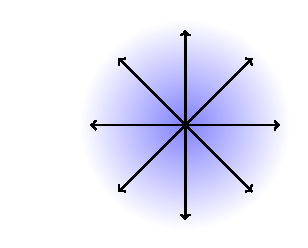
\includegraphics{figurer/omni-top.eps}
        \caption{Top view}
        \label{fig:omni-top}
    \end{subfigure}
    \begin{subfigure}[b]{0.55\textwidth}
        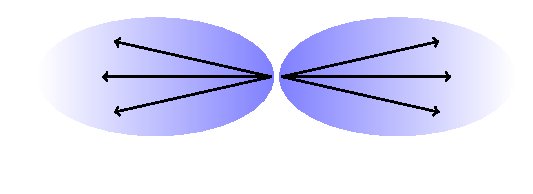
\includegraphics{figurer/omni-side.eps}
        \caption{Side view}
        \label{fig:omni-side}
    \end{subfigure}
  \label{fig:omni}
  \caption{Omnidirectional antenna}
\end{figure}

The absence of infrastructure implies their quick deployment and simple configuration.
The recent years have withnessed an increasing interest in WANETs, motivated by numerous both civil and military applications and by the continual progression in wireless technologies.
Digital battlefield, disaster management, luggage handling in airports, context aware computing and mobile commerce are examples of the growing list of potential applications of WANETs \cite{younis06}.

Fig. \ref{fig:communication} depicts different types of communication in wireless networks.
Consider a group of devices and a specific sender who initiates a signal transmission. 
A \emph{unicast} means that there is a single recipient.
Whenever the recepients are all the remaining devices within the group, we talk about a \emph{broadcast}.
Finally, a \emph{multicast} means that only some of the devices must receive the message. 
The remaining ones do not have to, but they can serve as intermediate devices forwarding the signal.

The wireless devices are typically heavily energy constrained due to the use of batteries as their energy source.
Energy conservation in WANETs is therefore plentifully pursued research topic.
Most of the energy is spent on signal transmission \cite{halgamuge09}, 
and so it is desirable to design energy efficient transmission protocols that also satisfy certain requirements imposed on a WANET.

Various levels of connectivity are required on WANETs.
However, from a practical point of view, a topology which is ``too connected'' would often cause communication interference to occur even between nodes that are fart apart.
Theoretical as well as practical experimental results suggest that the communication graph in WANETs should be as sparse as possible while preserving connectivity \cite{blough02}.

Models considered for WANETs are usually deterministic, that is, they assume that the nodes are fully reliable. 
In reality, the nodes are devices that may be subject to temporary or permanent failure due to technical damage or battery draining.
This fact leads to considering \emph{probabilistic} models whose aim is to capture the real world more plausibly by taking into account the uncertain character of nodes' availability.
Besides minimizing the power consumptions of the network, it is also required to guarantee a certain level of reliability over the whole network.

\subsection{Wireless Sensor Networks}

A related paradigm to WANET are Wireless Sensor Networks (WSN) which attracted a wide range of disciplines where close interactions with the physical environment are essential.
WSNs consists of tiny sensor nodes, which act as both data generators and network relays \cite{akyildiz10}.
Each node act as a senosr, a microprocessor and a transceiver.
Sensor nodes have usually a fixed position and are powered by batteries.
Data measured  by sensors are transmitted via wireless communication links

There are countless of sensor types including seismic, electromagnetic and acoustic, suggesting a broad area of practical application areas such as 
military, environmental, health, home and industrial applications.

Multiple sensors are typically integrated into higher-level topologies varying in complexity.
These topologies can be divided into flat and hierarchical architecture \cite{mcgrath13}.
In a flat (peer to peer) architecture, every node has the same computational and communication capabilities.
In a hierarchical architecture, simple sensor nodes operate in close proximity to their respective cluster heads which possess more processing capacity than an ordinary sensor node.

WSNs are often built using the following configurations \cite{mcgrath13}:

\begin{itemize}
\item \emph{Point to point topology.} Links two endpoints either permanently or with the possibility of switching.
\item \emph{Bus topology.} Each node is connected to a shared communication bus, in which a signal is transmitted in both directions. 
\item \emph{Linear topology.} Two way link between one node and the next one, with two terminating nodes.
\item \emph{Ring topology.} A networks set up in a circular fashion is similar to linear topology, but does not contain the terminating nodes.
\item \emph{Star topology.} Consists of a single central node such as hub or a switch to which every node in the network is connected. 
An intelligent central node is required as all data traffic flows through it.
This topology is one of the most common WSN topologies.
\item \emph{Tree topology.} A hierarchy of nodes where in the highest level of the hierarchy is a single root node connected to one or many nodes in the level below.
The processing and power requirements in nodes increase as the data moves from the branches towards to root node.
\item \emph{Mesh topology.} Nodes disseminate their own data and also act as relays to propagate the data from other nodes.
The mesh topology can be partially connected  or fully connected (where there is a connection between every two nodes.
\end{itemize}

\subsection{Combinatorial optimization problems motivated by WANETs}

As indicated above, energy conservation is a crucial requirement in the design of WANETs. 
Combinatorial optimization is endowed with methods suitable for this task. 
It is necessary to introduce a formal network model in order to apply suitable mathematical tools.

\subsubsection{Network Model}

A WANET is modeled by a complete weighted graph $(G=(V,E),p)$, where the wireless devices are represented by nodes in $V$. 
As no power limit is imposed on the nodes, a transmission can be established between any two nodes, and thus $G$ is complete.
The function $p:E\to \mathbb{R}^+$ indicates the power requirement for sending a signal along a certain edge.
This requirement depends on distance and environmental properties, and is given by  $p_{ij}=d_{ij}^\alpha$, 
where $d_{ij}$ is the Euclidean distance between the devices represented by vertices $i$ and $j$, and $\alpha$ is the constant environmental factor typically valued between 2 and 4. 
Some sources state the relation $p_{ij}=\kappa d_{ij}^\alpha$, where $\kappa\geq$ is a transmission quality parameter.
The transmission range of a node $i$ depneds on the power supply $P_i$ assigned to it.
The overal power assignment to individual nodes induces a directed transmission graph (see example in Fig.~\ref{fig:transgraph}. 
On the other hand, for a given transmission graph, the power assignment to a node corresponds to the longest outgoing arc.
\begin{figure}[htb!]
  \centering
  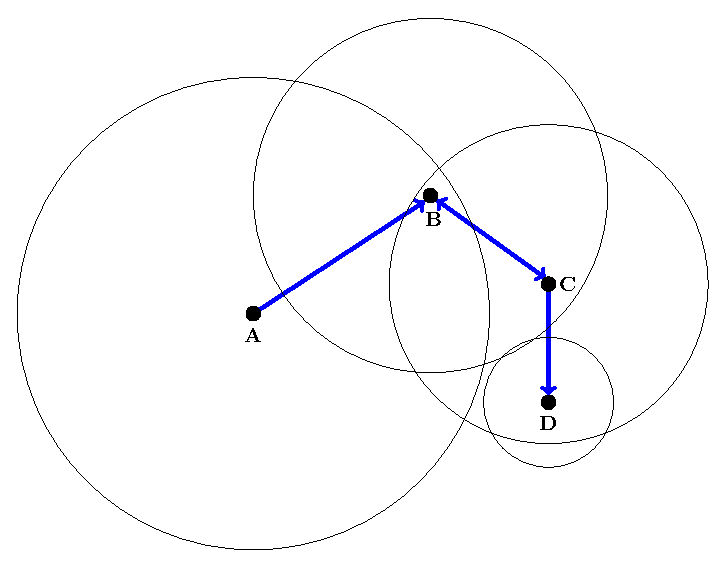
\includegraphics[scale=.8]{figurer/tran-graph.eps}
  \caption{Power assignment to nodes (circles)  and corresponding induced transmission graph (blue arrows)}
  \label{fig:transgraph}
\end{figure}
It is assumed that nodes are distributed in a Euclidean space, although it is also possible to consider more general variants..
In the following combinatorial problems motivated by WANETs, the task is to assign powers to individual nodes while satisfying certain criteria so that the overall power is minimized.
The total power is expressed by an objective function varying among the problem.

\subsubsection{Minimum Energy Broadcast}

The Minimum Energy Broadcast (MEB) problem consists of a set $V$ and a specified source $s\in V$, that is supposed to initiate a transmission.
All the remaining nodes must receive the signal via communication links induced by power assignment to the nodes.
\begin{problem}\label{prob:meb1}
Given a source $s\in V$, find a power vector $(P_1,P_2,\dots,P_n)\in\mathbb{R}^n$ of minimum sum s. t. 
there exists a path from $s$ to each $t\in V\setminus\{s\}$ in $G'=(V,E^P)$, where $E^P=\{(i,j)\in \vec{E}: p_{ij}\leq P_i\}$.
\end{problem}
An optimal solution differs for different transmission sources.
Hence, the nodes must by endowed with a mechanism that allows them to ajdust their power level for a corresponding transmission session.
This places demands on the computational capacity and technological solution of the nodes.
The advantage of this concept lays in the optimality of each broadcast session.

The directed graph induced by power assignmetns as defined in Problem~\ref{prob:meb1} is not necessarily an arborescence.
However, MEB could be stated slightly differently:
\begin{problem}\label{prob:meb2}
Given a source $s\in V$, find an arborescence spanning $G$ rooted at $s$ such that 
the sum over weights of the heaviest outgoing arcs of all nodes is minimized.
\end{problem}

\begin{observation}
The objective function value of a given instance is equal in Problem~\ref{prob:meb1} and~\ref{prob:meb2}.
\end{observation}

MEB  and has received a significant attention during the last two decades.
The problem has been introduced in \cite{wieselthier00}, where the authors propose a greedy algorithm called broadcast incremental power (BIP), which resembles Prim's algorithm for MST,
and improve it by a ``sweep'' operation removing unnecessary transmissions.
NP-hardness results for both general and geometric MEB are provided in \cite{cagalj02} by reduction from \textsc{Set Cover} and \textsc{Planar 3-SAT}, respectively.
In the former case, the network topology is represented by a generic graph with arbitrary weights, whereas in the latter a Euclidean distance is considered.
The special case where $\alpha=1$, i. e., where the edge weights correspond to distances between the endpoints belongs to $P$.
An optimal solution is determined trivially by assigning minimum power sufficient to reach all nodes in a single hop, regardless of the nodes' arrangement.


An approximation by MST has been investigated by several authors, e.g., in \cite{clementi01}.
After constructing an MST, the algorithm determines an orientation of arcs towards the leavs, starting from the source.
The last step is to assign power levels to each node according to the longest arc outgoing from that node.
This algorithm yields a solution no worse than 6 times the optimal one \cite{ambuhl05}.

The approximation ratio of an algorithm that builds an MST and assigns power levels to nodes ac
The algorithm that constructs a transmission tree based on MST first construct an MST, then 

A special case, assuming that there are $k$ adjustable power levels $w_{i,1},w_{i,2},\dots w_{i,k}$ at each node $i$ is studied in \cite{liang02}.
This problem remains NP-hard which is proved by reducing \textsc{3-CNF-SAT} to it.
In addition, \cite{liang02} contains an approximation algorithm for this version of MEB with a performance guarantee $\mathcal{O}(n^\epsilon)$ and 
time complexity $\mathcal{O}((k+1)^{\frac{1}{\epsilon}} n^{\frac{3}{\epsilon}}$ for $\epsilon\in \left(0,1\right]$.
Further restriction pursued in \cite{liang02} assumes that each node has the same adjustable power levels, i.e., $w_{i,l}=w_{j,l}$ for $1\leq l\leq k$ and $1\leq i,j\leq n$.
In this scenario, another approximation algorithm which delivers a solution within $\mathcal{O}(\log^3 n)$ times the optimum is devised.

Probabilistic MEB where a node reliability is considered has also been investigated.
Three ILP formulations of probabilistic MEB together with suitable solving methods are developed in \cite{montemanni08}.
Another study of ILP formulations and suitable valid inequalitis is pursued by \cite{barta10}.

A restriction of node locations can be imposed.
One example is a random grid network, where nodes are chosen independently and randomly from points of $\sqrt{n}\times\sqrt{n}$ square grid in the plane.
The probability distribution of existence of a node can be non-uniform.
A lower bound on the objective function is proved in \cite{calamoneri08} together with a near optimal construction method.
The 6-approximation of MST turns out to be too pessimistic for instances with restricted node locations which represent the real-life instances more closely.
Authors in \cite{flammini07} argue that the approximation ratio of MST algorithm can be considered close to 4 for practical instances.

Alternatively, a MEB instance can be defined by $G=(V,E)$ and its embeddding $\Phi(G)$ in a plane.
We recall from Section \ref{sect:back:graph} that an embedding of a graph in a plane assigns coordinates to nodes in a Euclidean plane.
These coordinates implicitly imply distance $d_{ij}$ between every two nodes $i$ and $j$.

The question addressed here is whether optimal solutions to various MEB instances have planar embedding.
By inspecting a large number of instances and their optimal solution, the planarity of the optimum cannot be guaranteed in general, even though in majority of cases, the optimum is indeed planar.
Any crossing in a graph (tree) involves 4 nodes that form a convex quadrilateral. 
We consider a quadrilateral $ABCD$ as depicted in Fig. \ref{fig:quad} with diagonals $AC$ and $BD$.
%A feasible solution to a MEB problem is an arborescence.
%The orientation of the diagonal edges can be arbitrary.
The \emph{adjacent sides} of a diagonal arc in $ABCD$ are the sides incident to the origin of the arc. 
So for example the adjacent sides of $(AC)$ are $AB$ and $AD$.
\begin{figure}[htb!]
  \centering
  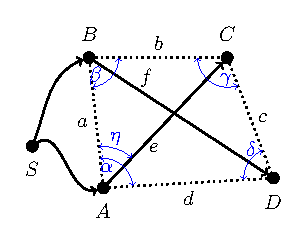
\includegraphics[scale=1.4]{figurer/quadrilat.eps}
  \caption{Example of a crossing in a solution to an instance of MEB}
  \label{fig:quad}
\end{figure}


\subsubsection{Range Assignment Problem}

In the range assignment problem (RAP) the task is to minimize the total power consumed under the constraint 
that adequate power is provided to the nodes to ensure a strong connectivity of the graph.
Formally, the problem is stated as follows:
%Therefore, only one broadcast tree is stored which is common for all possible sources.
\begin{problem}
Find a power vector $(P_1,P_2,\dots,P_n)\in\mathbb{R}^n$ of minimum sum s. t. the induced graph $G'=(V,E^P)$ is strongly connected, 
where $E^P=\{(i,j)\in \vec{E}: p_{ij}\leq P_i\}$.
%every where $E^P=\{(i,j)\in E: p_{ij}\leq P_i\wedge p_{ij}\leq P_j\}$.
\end{problem}
In \cite{kirousis00}, it is shown that for instances consisting of colinear points, there exists an algorithm that solves the problem to optimality in $\mathcal{O}(n^4)$.
The authors further prove by reduction from \textsc{Vertex Cover} that RAP in 3-dimensional Euclidean space is NP-hard,
and that there exists a $\mathcal{O}(n^2)$ time 2-approximation algorithm based on finding MST.
The results are strengthened in \cite{clementi99}, where it is proved that RAP is NP-hard for instances in a 2-dimensional Euclidean space, 
and that for 3-dimensional space, the problem is APX-complete, thus does not admit a PTAS unless P$=$NP.
An approximation algorithm improving the performance guarantee approaching 1.69 is presented in~\cite{calinescu02}.
A recent work \cite{carmi15} achieves an exact algorithm for the 1-dimensional problem that runs in $\mathcal{O}(n^2)$.


A further constraint requires that diameter of the transmission graph has to be at most some constant value $h$.
On a family of instances limiting the proximity of two nodes, this variant of RAP is in APX \cite{clementi01b}.
The 1-dimensional problem with restricted diameter (number of hops) has been studied in \cite{clementi03}, where the authors introduce an exact algorithm that runs in $\mathcal{O}(hn^2)$.

Another modifications requires symmetric communication links.
This version is often found in the literature under the abbreviation SRAP.
In a generalied version, weakly symmetric RAP (WSRAP), the symmetry requirement applies only to a pre-defined subset of edges.
Other edges which are not essential for connectivity are allowed to be unidirectional.
The motivation for studying WSRA stems from the observation that what is really important in the design of WANETs and WSNs is the existence of a connected backbone of symmetric edges \cite{santi05}.
Imposing symmetry does not change the complexity of the problem, which remains NP-hard in two and three-dimensional networks \cite{blough02}.

An obvious advantage of RAP over MEB is that a single transmission graph is constructed in RAP regardless of the source node.
However, this can lead to solutions optimal with respect to RAP, but for certain sources initiating the transmission, the solution can be too expensive.
The following problem with a more complicated objective function combines advantages of both RAP and MEB.

\subsubsection{Shared Broadcast Trees}

A feasible solution to the Shared Broadcast Tree (SBT) problem is any (undirected) spanning tree.
This concept is motivated by the intention of incorporating the frequency of use of each node for different broadcast sessions.
Every node can transmit a signal, but some are actively transmitting more often than others.
We assume that a node acts as a source with a uniform probability. 
A leave $l$ transmits a signal only when $l$ is a source, other intermediate nodes transmit more often as they also realay signals initiated in other nodes.

Observe that a forwarding node that received a signal does not have to send it back to the node from which the signal was received.
If the signal was received in a node $i$ from its most distant neighbor node $i_1$, it has to be forwarded to nodes that have not received it yet along the link to the second most distant node $i_2$..
Due to the wireless advantage, all other neighbor nodes closer than $i_2$ receive it as well.
Conversely, if the signal was received by $i$ from a neighbor node different from its most distant neighbor $i_1$, node $i$ has to forward it to $i_1$. 
It is therefore evident that $i$ does not have to always transmit with the power corresponding to the most distant neighbour.
It transmits either with power level $p_{ii_2}$, if the signal came from the most distant node $i_1$, or with power level $p_{ii_2}$, otherwise.
The situation is depicted in Fig~\ref{fig:objexp}.
\begin{figure}[htb!]
  \centering
  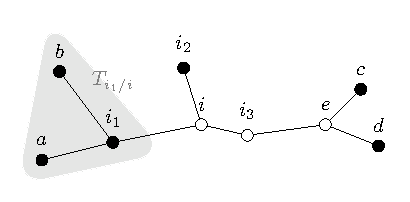
\includegraphics[scale=1.4]{figurer/objexp.eps}
  \caption{Example instance explaining power levels necessary for transmitting a signal from different sources}
  \label{fig:objexp}
\end{figure}


Consider an arc $(i,j)$ in a solution $T$ to SBT.
Let $T_{i/j}$ denote the subtree of $T$ consisting of nodes whose path to $j$ contains $(i,j)$. 
A node $i$ in $T$ contributes to the objective function by the expression $c_T(i)$ as follows:
\begin{equation}
c_T(i)=|T_{i_1/i}|p_{ii_2} + |T\setminus T_{i_1/i}|p_{ii_1}.
\end{equation}
We can also regart $c_T(i)$ as a weighted arithmetic mean of $i$'s power levels, with weights corresponding to the number of nodes whose signal is transmitted using the corresponding power level.
The objective function is to minimize overall nodes' contributionss, that is,
\begin{equation}
c(T)=\left\{\sum\limits_{i\in V}c_T(i) \right\},
\label{eq:sbtcost}
\end{equation}
The problem under study is thus defined as follows:
\begin{problem}
Find a tree $T\subseteq G$ spanning $D$ minimizing \eqref{eq:sbtcost}.
\end{problem}

\emph{Remark:} The requirement that a solution must be a tree is necessary due to the nature of the objective function.

Like in MEB, an optimal solution to SBT does not guarantee a planarity of the resulting tree, although vast majority of instances are planar. 
As an example of non-planar optimum we state the instance depicted in Fig~\ref{fig:sbt-nonplanar}.
\subsubsection{Non-destination nodes}

Additional assumption of the existence of nodes that never initiate any transmission is a natural extension of all the problems described above.
It is similar to the generalization of MST which leads to the Steiner minimum tree problem.
In MEB, RAP and SBT, nodes that do not have to be part of the network are also allowed. 
These nodes never initiate any transmission, nor they have to receive any signal.
They can act as intermediate nodes relaying the signal, if improves the respective objective function value.
Apart from the weighted graph $G=(V,E,p)$, the set of nodes $D\subseteq V$ called \emph{destinations} is also a part of the input.
Nodes in $V\setminus D$ are referred to as \emph{non-destinations}.

In MEB, the presentce of non-destinations leads to the Minimum Energy Multicast (MEM) problem introduced along with MEB in \cite{wieselthier00}.
It is easy to see that MEM is NP-hard by reducing the Steinter tree problem to it.


The following section gives a particular attention to the multicast version of SBT.

\subsection{Shared Multicat Trees}

The Shared Multicast Tree (SMT) problem is a natural generalization of SBT.


\section{Minimum Broadcast Trees}\label{sec:mbt}

\section{Multi-Agent Path Finidng}\label{sec:app}

In multi-robot path finding (MPF) we consider an environment with several identical moving entities referred to as 
\emph{agents}. Source and target locations are uniquely determined for each agent. The objective
is to find a route for every agent from its source to its target.
Agents must not collide with obstacles and other agents that are also moving along
planned routes towards their own targets.
The environment is modeled as an undirected graph, where the agents are placed in the vertices, and move along the edges from one vertex to another. 
Continuous time is divided into discrete time steps, where the relocation of an agent from one vertex to its neighbor takes exactly 1 time step.

Different variants and restrictions have been studied.

\emph{Muliti-agent path-finding} (MPF) \cite{source1}  supposes a group of agents in a given
environment, where initial and target positions are determined for each agent.
All individual agents must avoid collisions. Movement of the agents is carried
out in discrete time steps. Agent can shift from one vertex to its neighbor on
condition that the neighbor is either unoccupied or is being left by other agent
in the same time step. At most one agent is allowed to pass an edge within one
time step. That is, agents are not allowed to exchange their positions within one
time step.

\emph{Pebble motion on graphs} \cite{source1,source2} is a very similar problem as MPF. It can
be regarded as a restricted variant of MPF. The difference consists in rules for
movement. While MPF enables entering a vertex that is simultaneously being
left by other agent, such transfer is not permissible in pebble motion. As an
illustration we can mention 15 puzzle also known as Lloyd’s 15 \cite{lloydXX}.

\emph{Cooperative Path-finding} \cite{cpf} is a special case of MPF where each agent is
assumed to have a full knowledge of all other agents and their planned routes.
Precisely speaking, solving algorithm can take into account paths planned for
agents that were processed earlier, and adjust paths searched later according to
them.

\subsection{Scenarios with adversaries}

\subsubsection{Adversarial Cooperative Path Finding}

\subsubsection{Area Protection Problem}

\subsubsection{Area Protection Problem with Communication maintenance}

